\lhead{\emph{Implementation}}

% ***************************************************************************
\chapter{Implementation} \label{chapt:implementation}
% ***************************************************************************

All the above mentioned techniques appear to be efficient only under specific constrains. In our scenario none of them can be applied directly and we have to find a more suitable procedure for this project. \\
Even for humans, manually calibrating these point clouds is a hard task. Due to the lack of overlapping, it is difficult to notice whether a transform is wrong or not when focusing only on closest points matching (similarly to \acrshort{icp} algorithm). However, knowing that this is a scene containing large planes that can be seen in both views, we naturally tend to estimate the correctness of the registration by judging if the final result is coherent or not, if the planes are aligned or not (this is similar to plane matching). \\
Both this methods are used by our brain in the same time to evaluate how coherent is the matching. In the same way, our program have to mix both techniques to get the best result. Some similar approaches are described in the literature. The registration can be performed in one step, mixing keypoints (2D or 3D) and plane primitives as implemented in \cite{mdou2013} and \cite{ytaguchi2013} or in 2 steps \cite{pkim16}, in this case keypoints are used as a robust method to register 2 similar point clouds while plane matching is used in a second registration process to improve point cloud alignment. This 2 steps methods can't be applied to low-overlapping point clouds because, as explained in chapter \ref{ch:soa}, both methods can't be applied separately in this case.\\
\newline
As we have seen, the most reliable information we have is given by planes that are visible from both cameras. The first step would then be to identify as many planes as possible. Depending on how many planes we can match, the remaining degrees of freedom will be fixed with keypoints matching. \\
In this scene two mains plane can be identities, which means only one translation remains to be solved. Thus, only one point is needed, in theory, to solve the registration completely. The problem is that the point cloud quality doesn't let us find perfect matches. I will then try to identify as many matches as possible so that, on average, the error is lowered. \\
\newline
As explained previously, both registration using points matching or planes matching works in a similar way. It is still needed to adapt these equations to be able to find the transformation that minimize both points and planes distance in the same time. 

\section{Preprocessing}

Before implementing any registration technique, few preprocessing steps are required to prepare data, fasten computation and improve 

\subsection{Downsampling}

The first thing that appears is that point clouds are really heavy data structures and processing them will require a huge computation power. To be able to perform fast computation on point clouds I started by sub-sampling the point clouds to reduce the number of points.

\begin{figure}[h!]
\centering
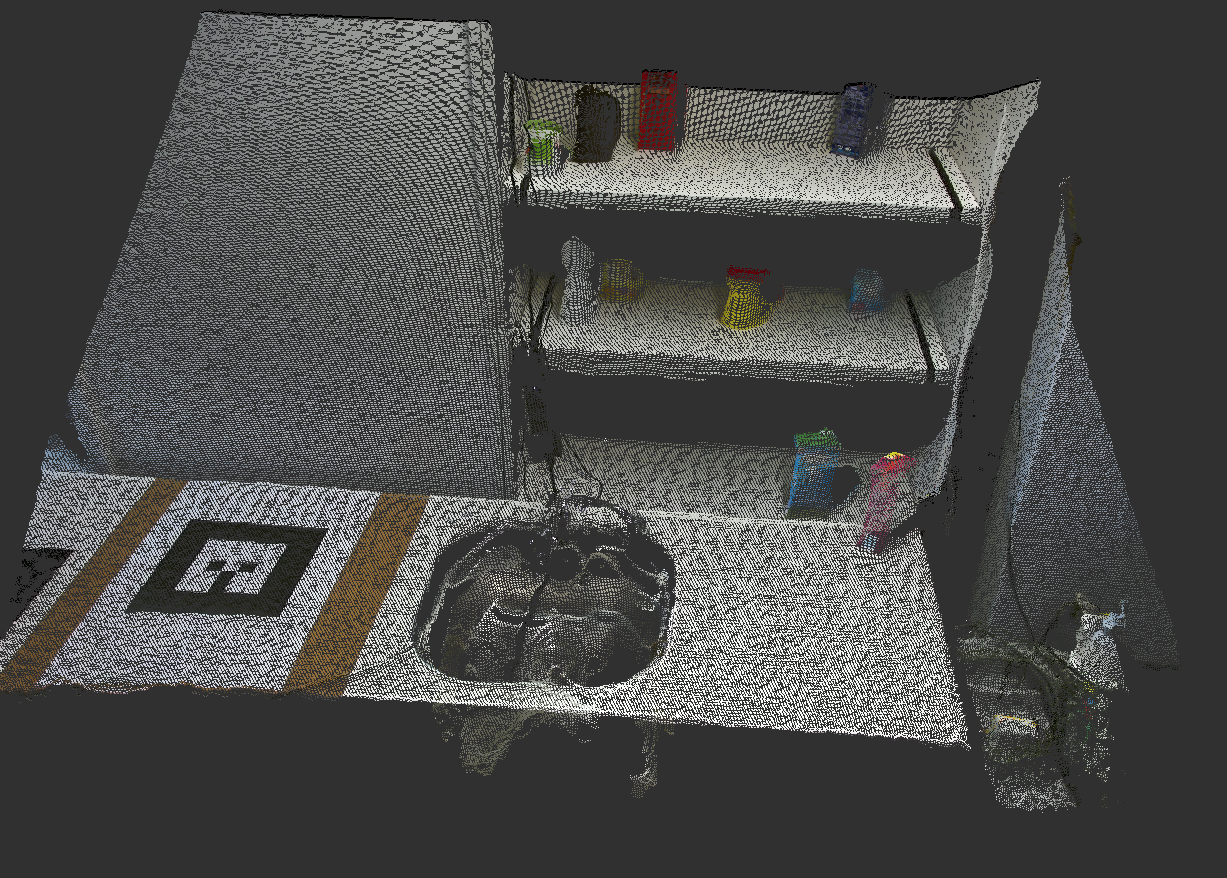
\includegraphics[width=\textwidth]{images/fullpc.png}
\caption{Full point cloud (16.588.800 points)}
\label{fig:fullpc}
\end{figure}

\begin{figure}[h!]
\centering
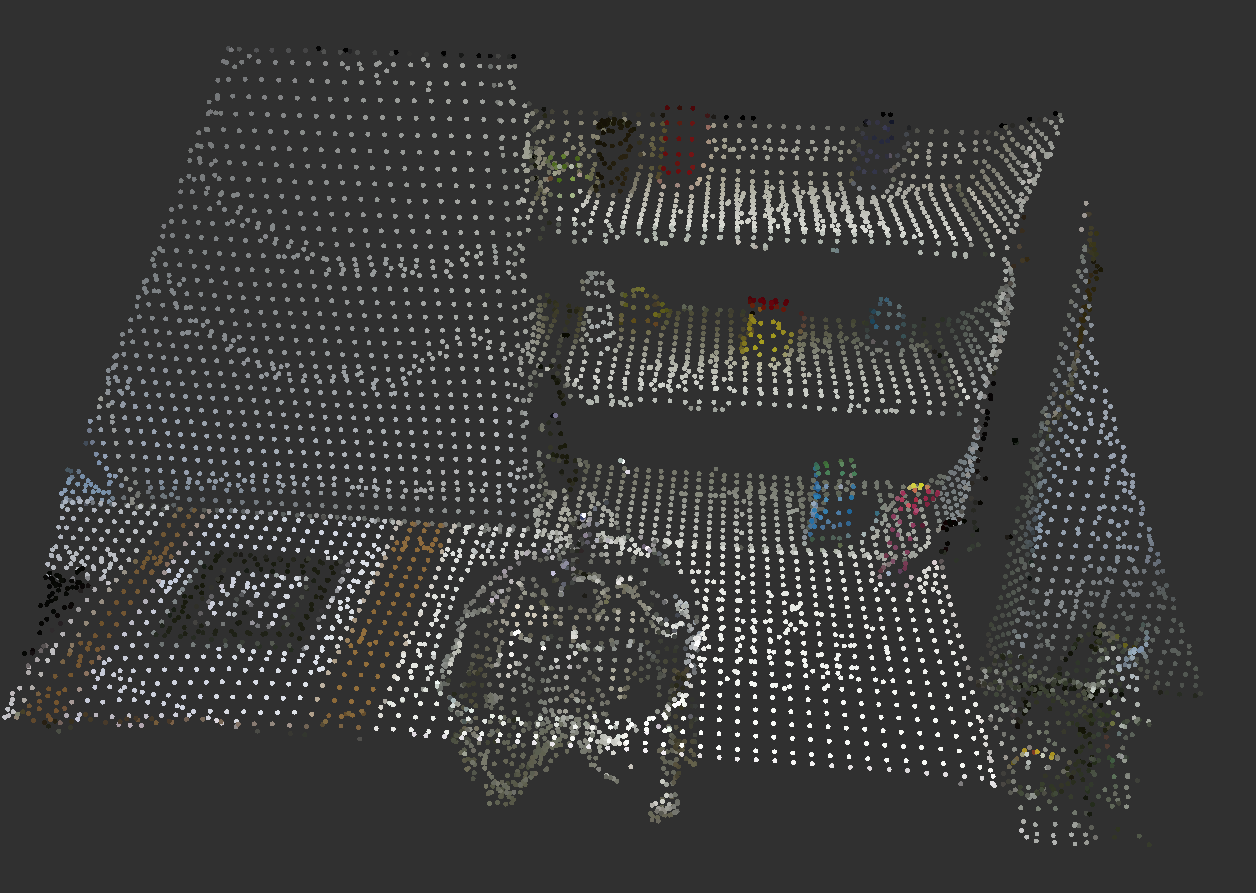
\includegraphics[width=\textwidth]{images/subsampled.png}
\caption{Sub-sampled point cloud (size: 3cm, 100k points)}
\label{fig:subpc}
\end{figure}

Sub-sampling allow to significantly decrease the size of the data to process by picking equally spaced points which makes the final result keeping most of the relevant information of the point cloud.

The sub-sampling size can be chosen to adapt the precision/performance ratio (fig. \ref{fig:sub_size}).

\begin{figure}[h!]
\centering
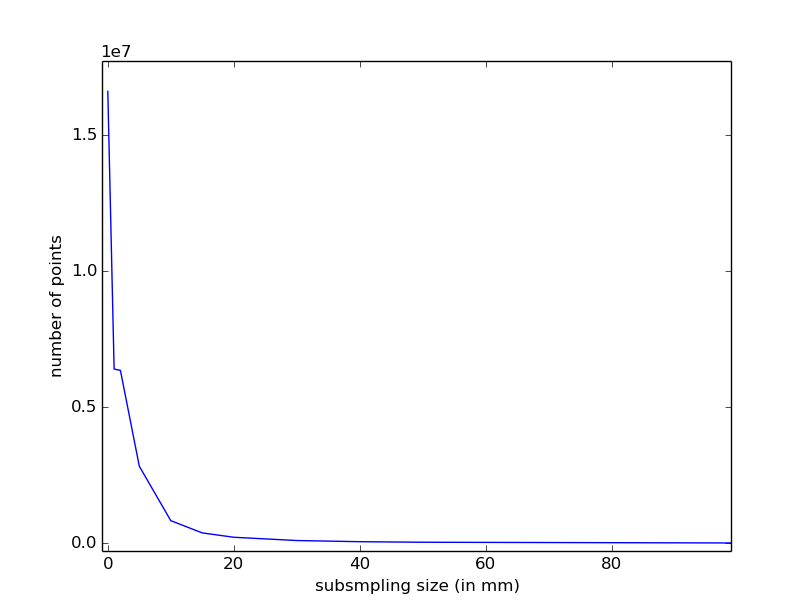
\includegraphics[width=\textwidth]{images/subsampling_size.png}
\caption{Example of evolution of the point cloud size against sub-sampling size.}
\label{fig:sub_size}
\end{figure}

\subsection{Cutting}

Another way to reduce the point cloud size is to cut it to remove non useful parts. This obviously requires to have some knowledge of the information received by the camera and will not be applicable in the case of a new unknown scene. However, cutting the point cloud will helps to quickly implement some registration techniques and will be used for testing and debugging purpose. In our project, when we try to fix only small camera displacements, we already have some rough knowledge on the scene. We can, for example, cut $z=0$ points that corresponds to the floor, using some margin threshold we can reasonably except that the floor will be cuted without losing any points on the table ($z=80cm$) unless the camera angle has been greatly modified.

\begin{figure}[h!]
\centering
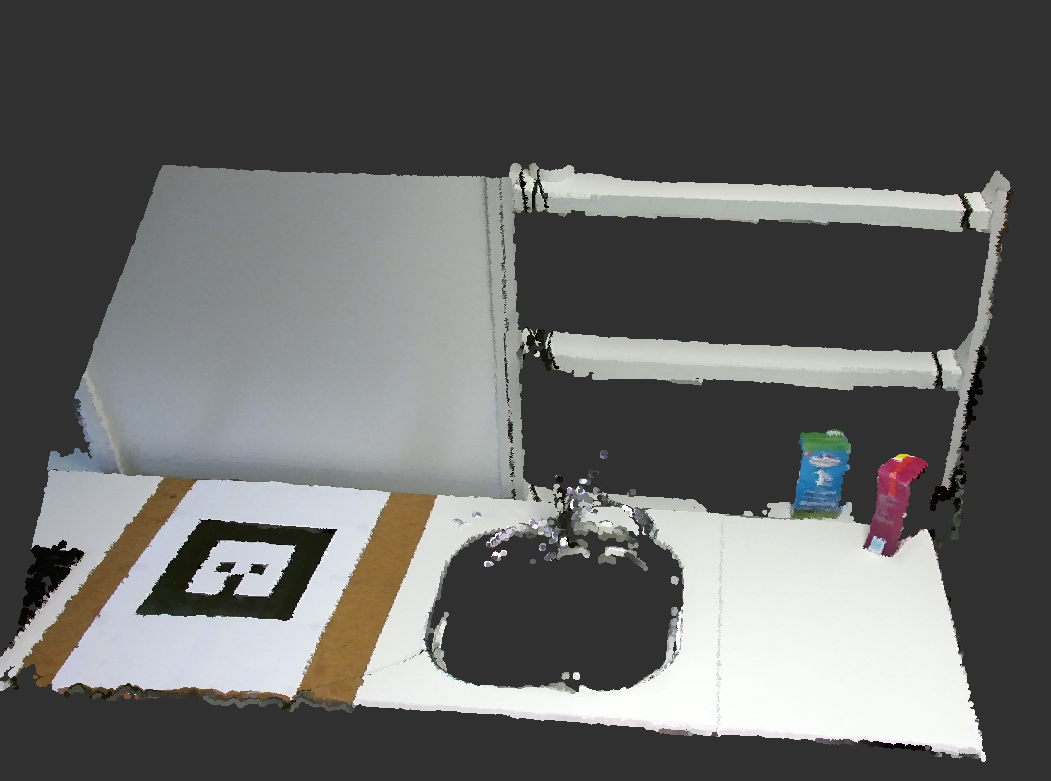
\includegraphics[width=\textwidth]{images/cut.png}
\caption{Example of point cloud cut using knowledge on the experiment environment.}
\label{fig:cut}
\end{figure}

In this example I cut the point cloud to keep only the points inside the working area.

\subsection{Filtering}

Finally, point cloud filtering is also a way I considered to decrease the size of the point cloud. I used radius filtering to delete outliers (points that don’t have enough neighbors inside a chosen radius). However this filtering was needing a lot of computation time compared to the small improvement it provides in this case. I no longer use this filtering in the preprocessing stage. 

\section{Plane Detection}

The first processing step consists in extracting planes from the point clouds. I am using \acrshort{ransac} (detailed in alg. \ref{alg:ransac}) algorithm to detect the most relevant plane of the cloud. I used \acrshort{pcd} \gls{library} implementation of this algorithm to perform fast plane detection.

When we find a good model, if we note $w$ the ratio between the number of inlying points and the total number of points, we can estimate the number of iterations needed to be confident enough that a correct model has been found. For example if we iterate the algorithm $k$ times, success probability $p$ can be written:
\[
    (1-w^3)^k=1-p
\]
The minimum number of iteration is then:
\[
    k=\frac{log(1-p)}{log(1-w^3)}
\]

In our setup, we can check how many iterations are needed. In the worst case, the first plane we want to detect is only $25\%$ of the point cloud. It means that using 500 iterations, we have less than $0.1\%$ chance not to find a good model. 

When the first plane is extracted, we can continue by subtracting inliers from the point cloud and apply again the \acrshort{ransac} algorithm, by iterating these steps I can extract as many planes as needed and they are extracted ordered by decreasing size. The idea is then to apply this plane detection on each point cloud in order to match these planes between both clouds. 

\section{Plane Matching} \label{sec:plane_matching}

Plane matching consists in matching as many planes as possible between different cameras. These planes should be matched when they correspond to the same plane in the real scene. Based on \cite{mdou2013}, I implemented a plane color histogram matching as follow. \\
By extracting the color data from each point of point cloud subsets corresponding to a plane we can compute a color histogram representing color distribution in a given color space. This space can be \acrshort{rgb} or \acrshort{hsv} and can be computer for 3 1D color channels (fig. \ref{fig:color_hist}) or for a 3D color space (fig. \ref{fig:3D_hist}).

\begin{figure}
   \begin{minipage}[t][6cm]{0.33\linewidth}
        \subfloat{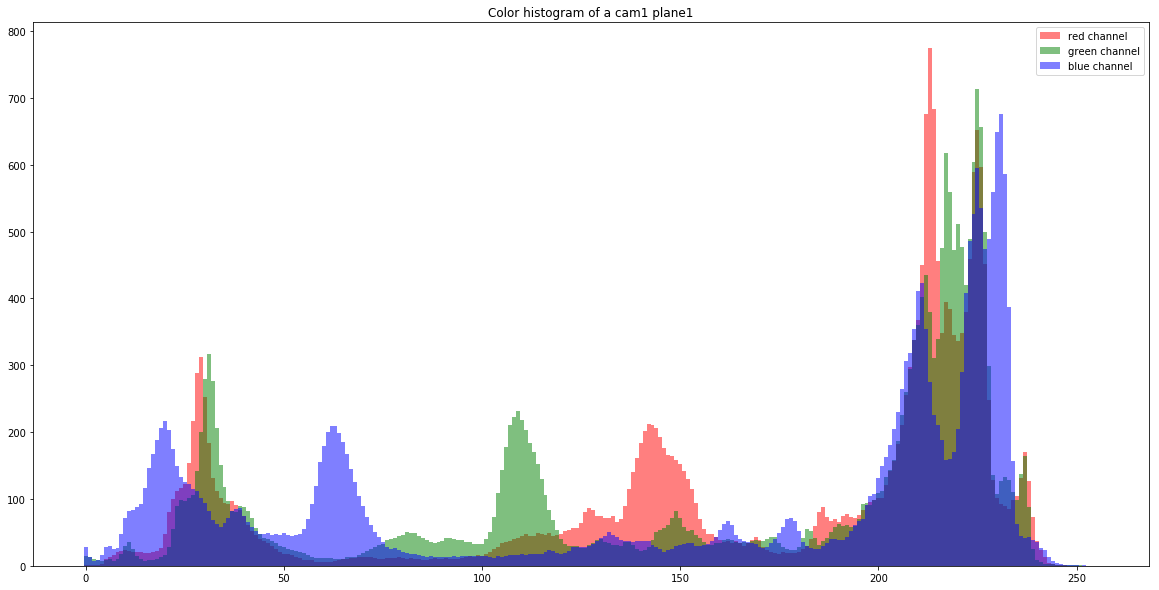
\includegraphics[width=\textwidth]{images/c1p1.png}}
        \subfloat{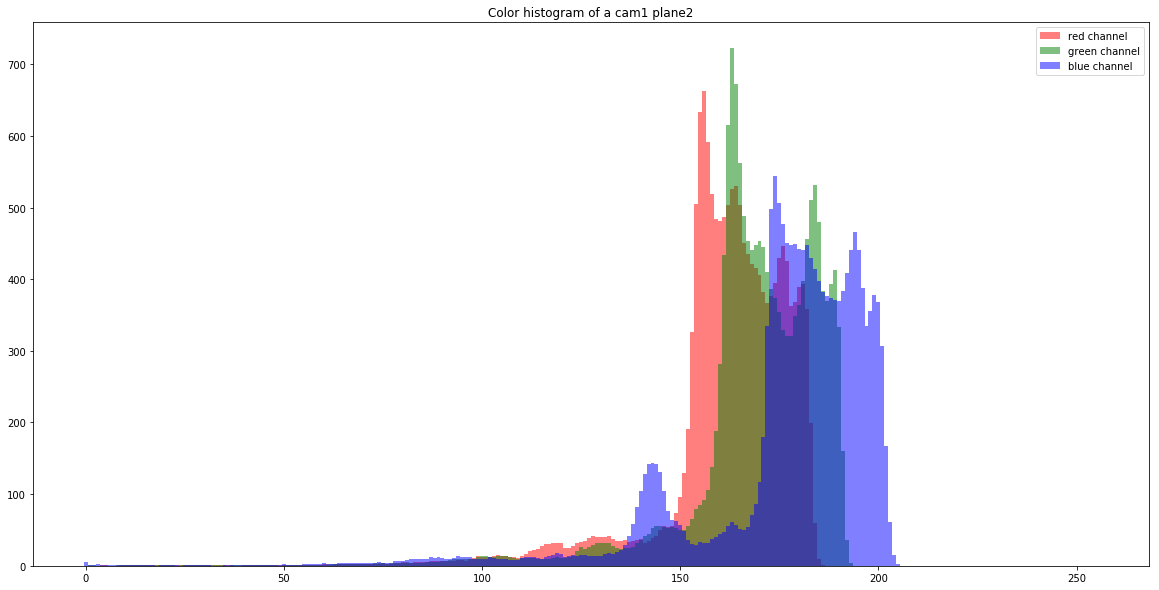
\includegraphics[width=\textwidth]{images/c1p2.png}}
        \subfloat{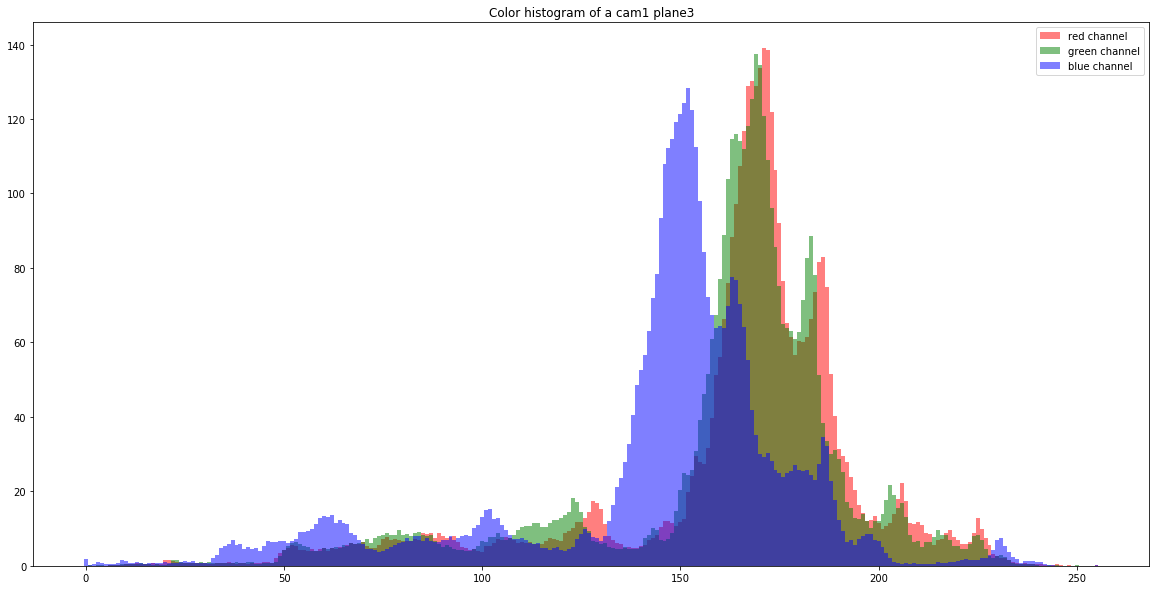
\includegraphics[width=\textwidth]{images/c1p3.png}}
    \end{minipage}%
    \begin{minipage}[t][6cm]{0.33\linewidth}
        \subfloat{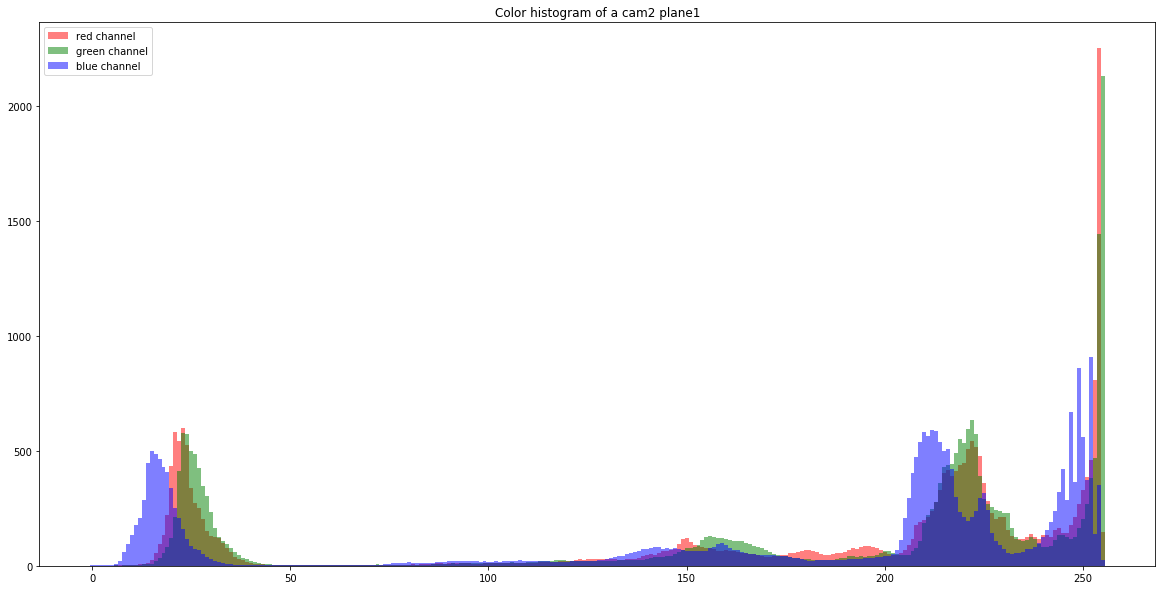
\includegraphics[width=\textwidth]{images/c2p1.png}}
        \subfloat{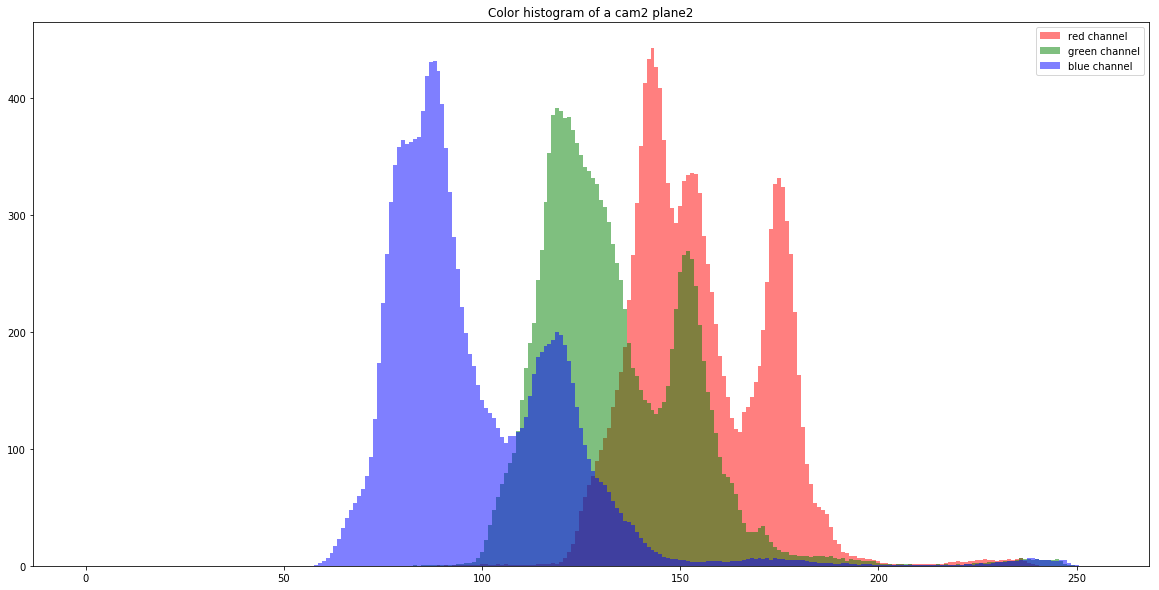
\includegraphics[width=\textwidth]{images/c2p2.png}}
        \subfloat{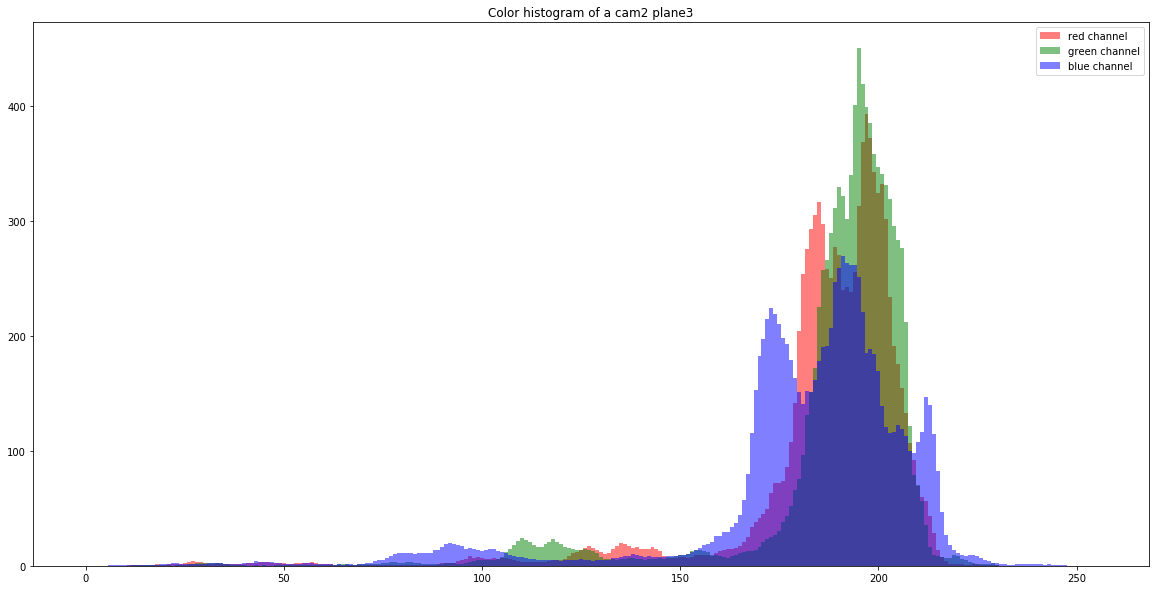
\includegraphics[width=\textwidth]{images/c2p3.png}}
    \end{minipage}
    \begin{minipage}[t][6cm]{0.33\linewidth}
        \subfloat{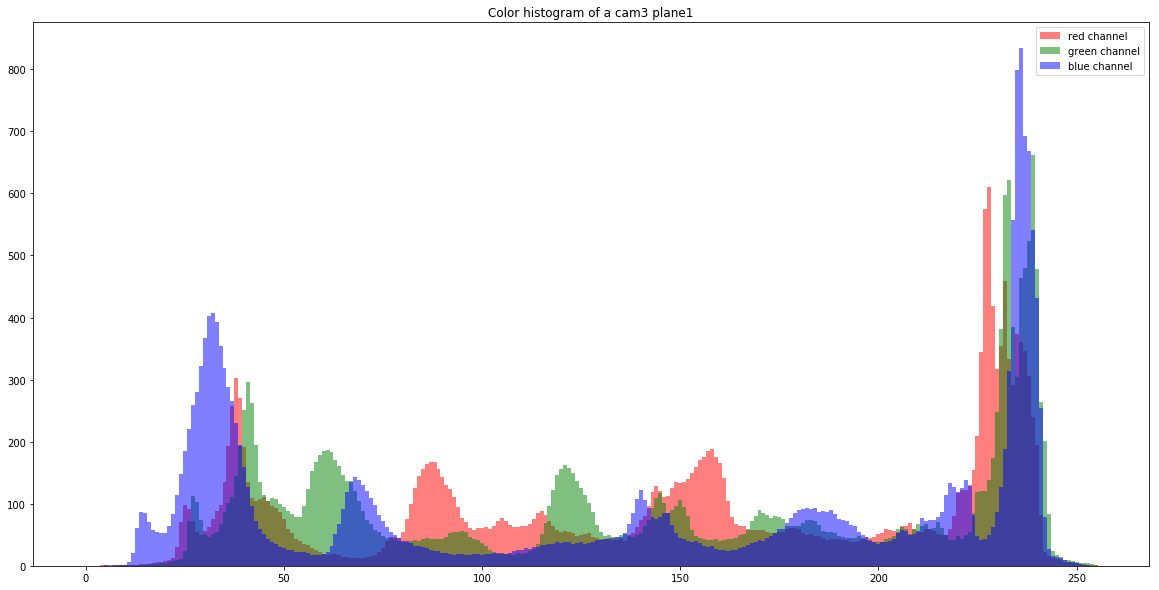
\includegraphics[width=\textwidth]{images/c3p1.png}}
        \subfloat{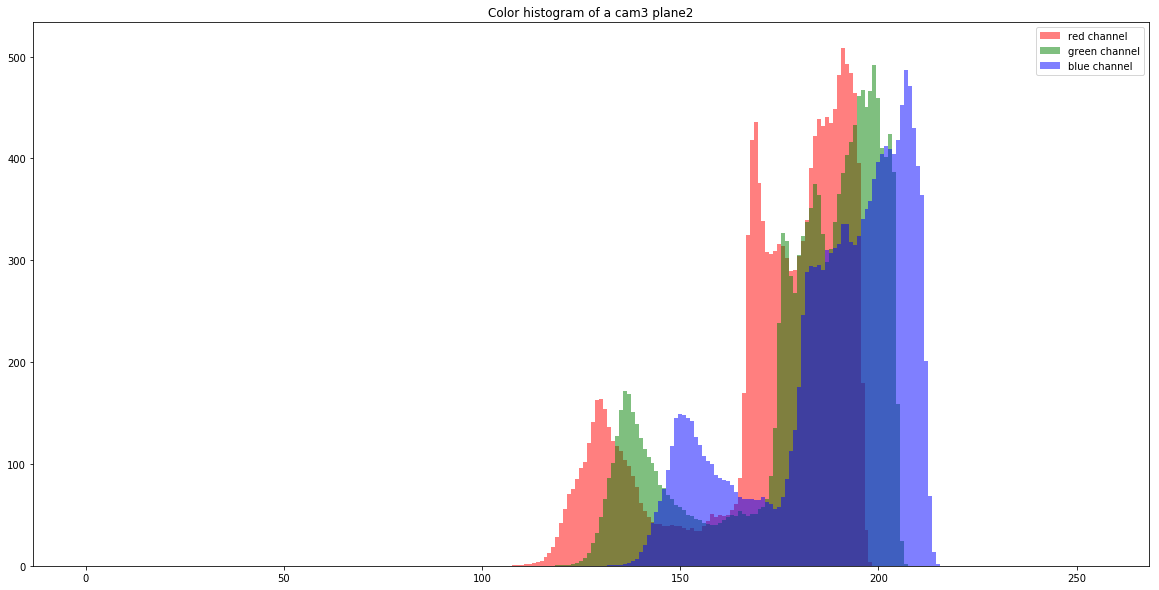
\includegraphics[width=\textwidth]{images/c3p2.png}}
        \subfloat{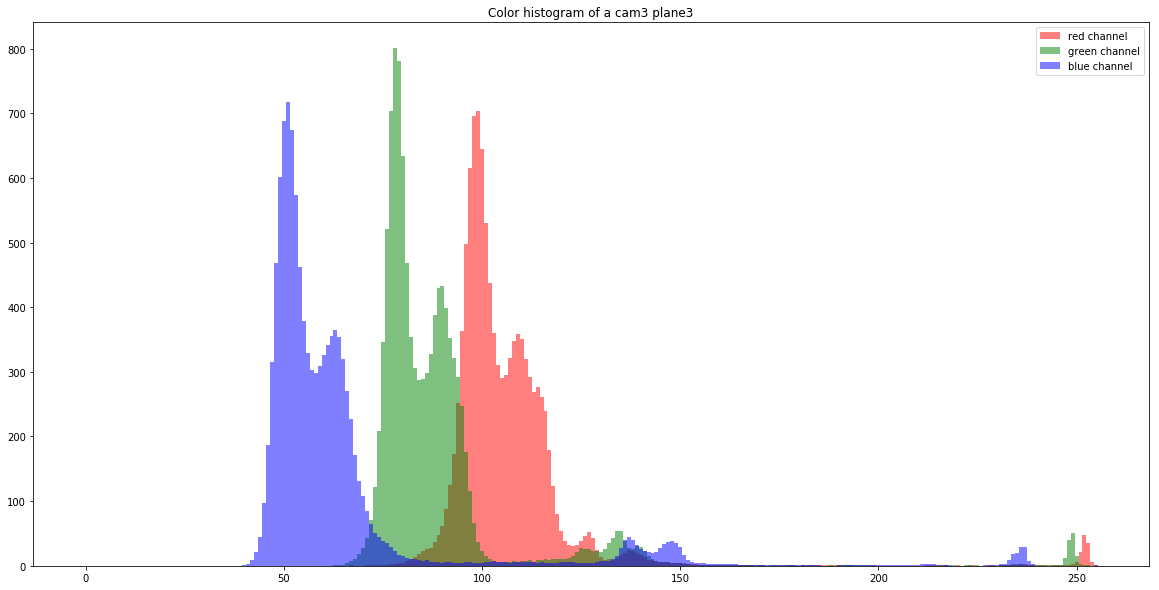
\includegraphics[width=\textwidth]{images/c3p3.png}}
    \end{minipage}
    \vspace{4em}
    \caption{Planes RGB color histograms computed for 3 cameras on 3 different planes (table, wall and wooden plate), each line represents a plane, each column represents a camera. }\label{color_hist}
\end{figure}

\begin{figure}[h!]
\centering
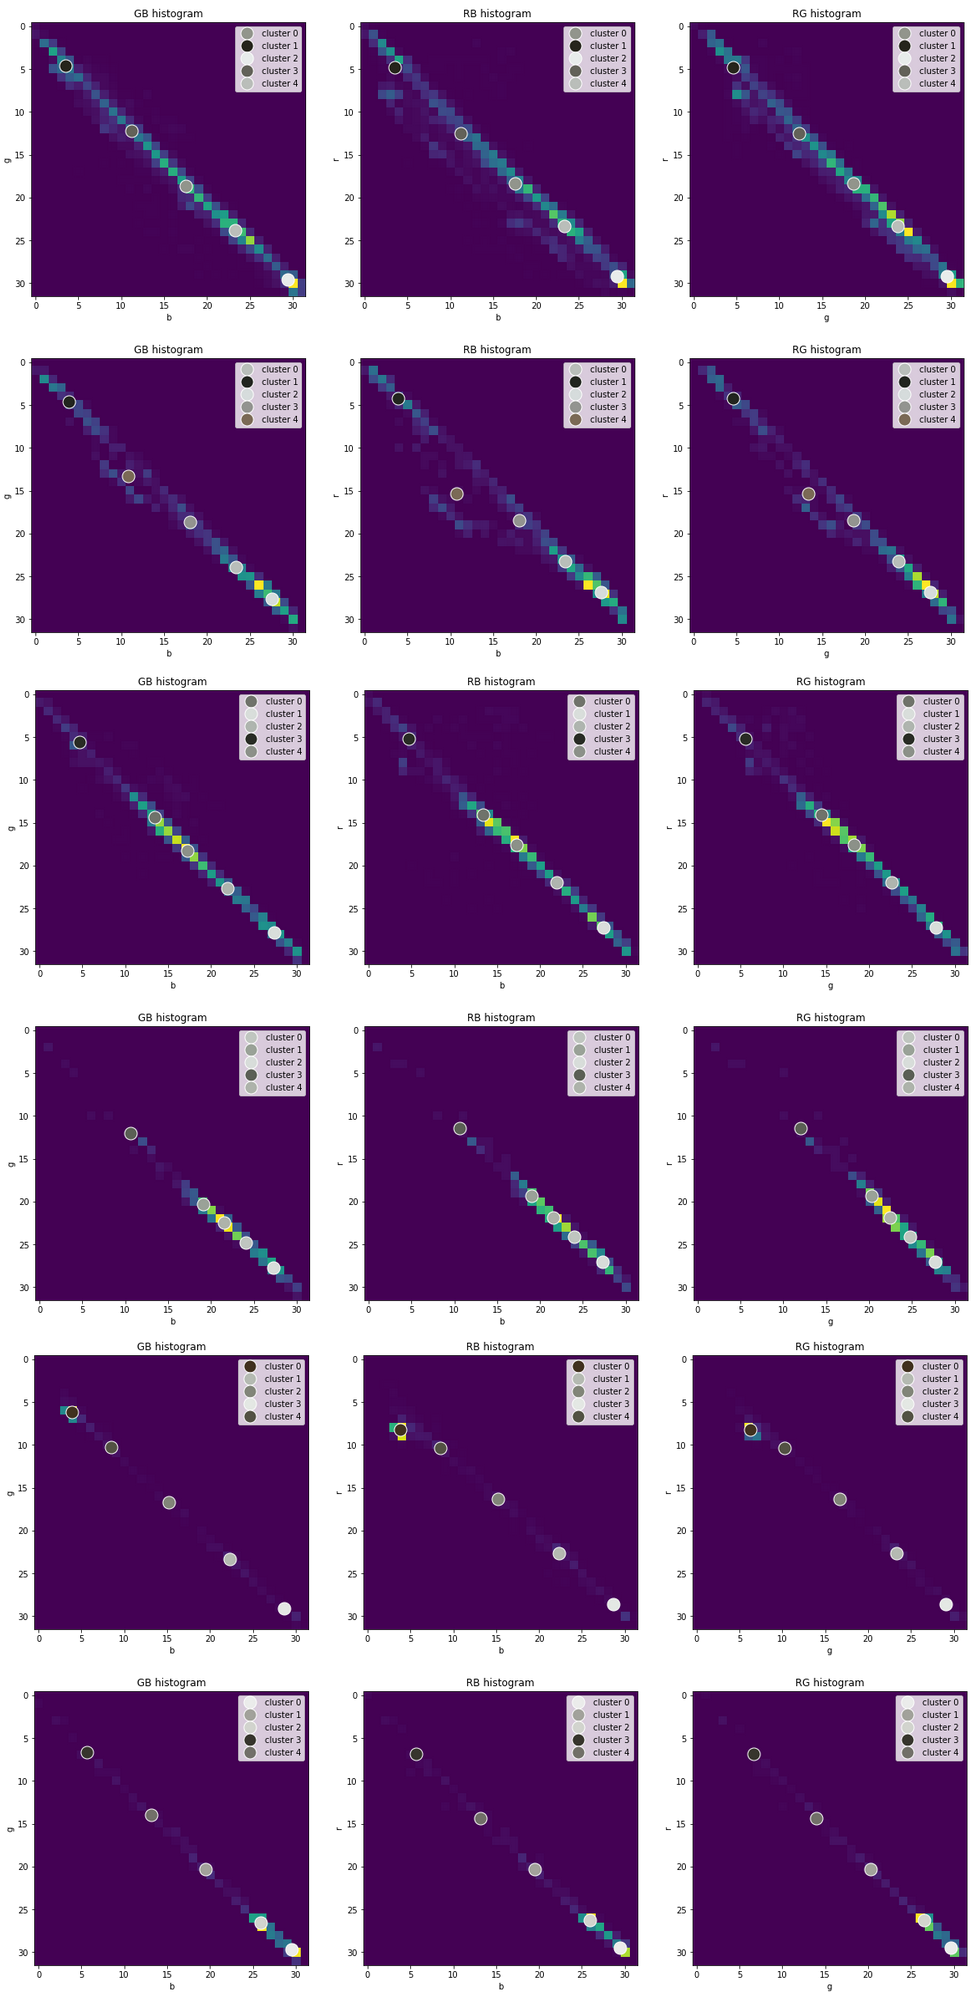
\includegraphics[width=0.8\textwidth]{images/kmeans_3D_hist.png}
\caption{2D projections of 3D color histograms for each planes. Lines correspond to plane 1 seen from cam1 (line 1) and from cam2 (line 2) then plane 2 (lines 3, 4) and plane 3 (lines 5, 6). Centroids of K-mean clustering (k=5) are shown with the corresponding color.}
\label{fig:3D_hist}
\end{figure}

Depending on the type of histogram different distance metrics can be used. As suggested in \cite{mdou2013}, overlapping areas can be computed for 1D histograms. I also performed K-means clustering on 3D histograms to determine the k=5 most common colors in each plane, it can be seen on fig. \ref{fig:3D_hist} that all colors are mostly grey which makes the matching difficult. It is then easy to compute a distance (Euclidian or Manhattan distance) between these centroids to find best matches. Given a plane color histogram from plane 3, I plot the distance to other planes color histograms captured from the 3 planes on both cameras on fig. \ref{fig:color_dist}. \

However, none of these techniques achieves a robust matching due to the very similar colors in each plane and the very low number of common points shared by planes seen from different cameras.
    
\begin{figure}[h!]
\centering
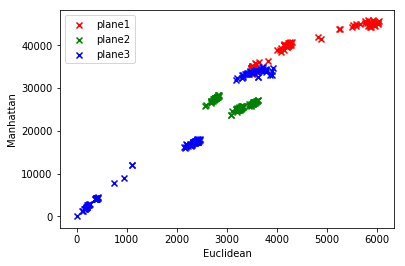
\includegraphics[width=0.6\textwidth]{images/dst_hist.png}
\caption{Distance between K-Means centroids computed between planes color histograms from different cameras and time and a color histogram from plane 3 seen from cam 1.}
\label{fig:color_dist}
\end{figure}



As explained in section \ref{sec:plane_detection}, I also tried to use \acrshort{pcl} \acrshort{vfh} global descriptor for matching planes. This techniques didn't allow me to match planes robustly neither.
For this reason, I preferred to match planes by comparing normals, this technique doesn't rely on the later use of plane matches and is simple to implement. The only requirement is not to have a huge orientation difference between cameras. This means we need a prior knowledge of the rotation between cameras ($\pm 45^\circ$). Given 2 planes $\pi_1=(n_1^\top, -\rho_1)$ and $\pi_2$ which normal vectors $n$ are chosen such that their product is positive, the metric $f$ I use for matching is the following, with an arbitrary $\alpha = 1\:m^{-1}$:
\[
    f(\pi_1, \pi_2) = n_1\cdot n_2 - \alpha \left | \rho_1 - \rho_2 \right |
\]

The first term $n_1\cdot n_2$ measures the cosine of normals angle between 0 (when they are perpendicular) and 1 (when they are parallel). The second term lowers this value if planes are far from each other. It allows planes to match with the right plane instead of an other parallel one.

\section{Keypoint Extraction}

As explained in sec. \ref{sec:plane_detection}, we usually don't detect 3 non-degenerated planes in the point cloud, especially when the overlapping is small. To solve this problem I am adding knowledge from the keypoints detection as done in \ref{sec:3dkp}. Method to estimate the transform from mixed data of planes and points is detailed in the next section.

Keypoints information is less precise than planes so we may want to give more importance to planes matching and use only keypoints to fix the last degree of freedom. We can define a weight between planes and points terms in the transform estimation equation. That way we give more importance to information provided by planes. However, we actually want to trust only planes for most of the degrees of freedom and use points matching only when it is needed. For example, we usually detect planes in 2 different orientations as we can see on fig. \ref{fig:planes_scene}, which means we still have to fix one degree of freedom (translation). We want, in this case, to use keypoints only to determine this translation. To achieve this, I compute the intersection direction of planes and I project keypoints along this vector. That way, keypoints will only contribute to modify the translation part of the transform in this direction as shown on fig. \ref{fig:proj}. By doing this we ensure that keypoints matching doesn't introduce a bigger uncertainty for rotations and translations that are already accurately determined by planes.

\begin{figure}[h!]
\centering
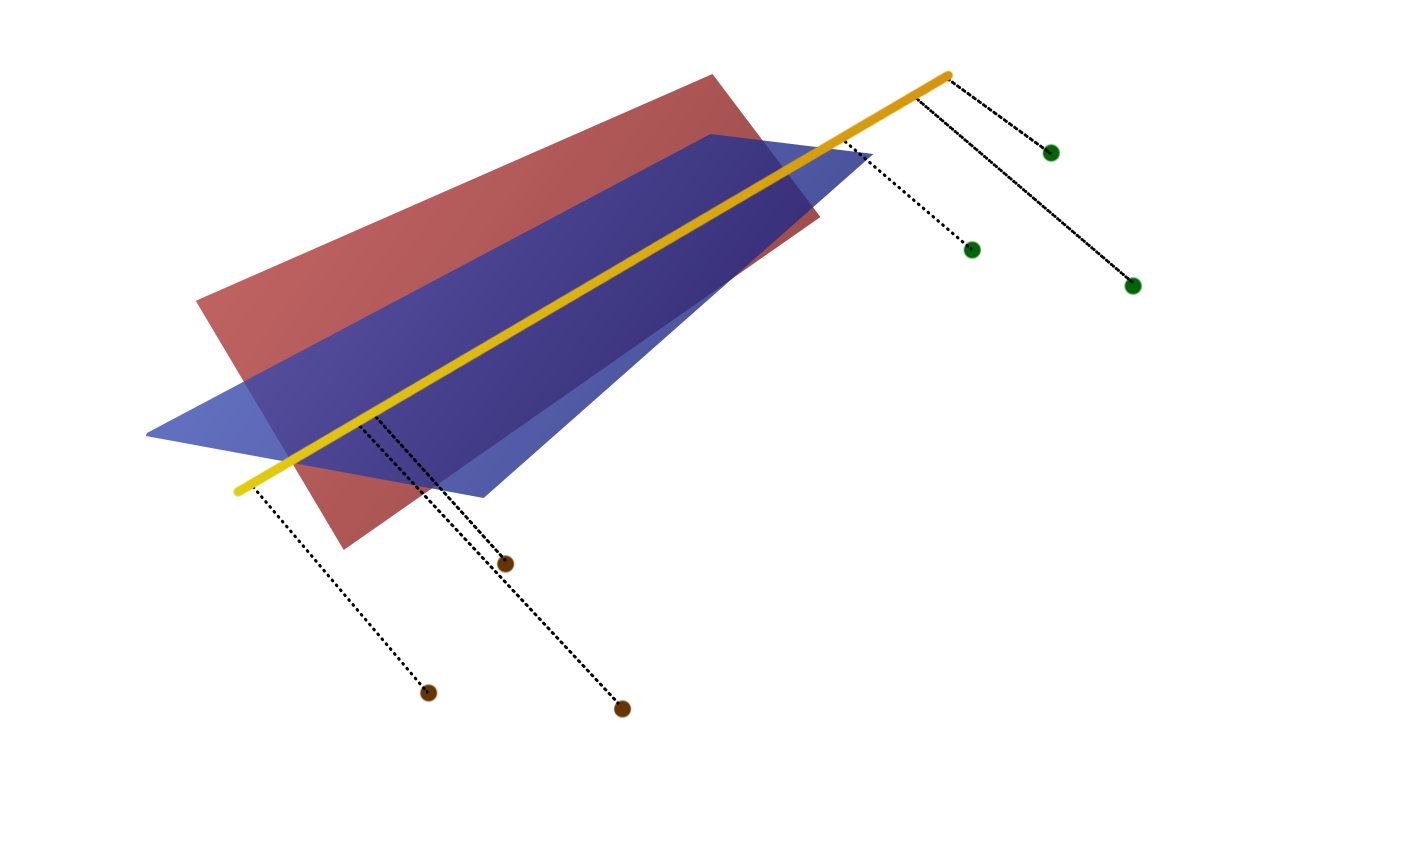
\includegraphics[width=\textwidth]{images/proj.png}
\caption{Projection of keypoints on plane intersection axis.}
\label{fig:proj}
\end{figure}

\section{Transform Estimation}

My implementation of transform estimation using both matched points and planes is based on equations derived in \cite{ytaguchi2013}. As described in \cite{khoshelham2016}, we can compute distances between planes (the value that should be minimized) in two different ways:

\begin{itemize}
    \item Plane to Plane, which is an arithmetic distance obtained by comparing plane equations. It is composed by the vector distance between plane normals and the scalar distance between $\rho$ parameters. 
    \item Point to Plane, a geometric distance obtained by averaging point to plane distances from one plane to another.
\end{itemize}

I am using the plane to plane distance since it is by far the fastest to compute.
My implementation is then based on these equations derived in \cite{khoshelham2016}. Equations are similar to the ones detailed in sec. \ref{subsec:transf_est} but we are adding terms (in red) related to plane normals. Resulting equations are then a generalized form of the equations from sec. \ref{subsec:transf_est} and \ref{sec:plane_detection}:

\[
R=U\begin{pmatrix}
1 &  & \\ 
 & 1 & \\ 
 &  & det(UV^\top))
\end{pmatrix}V^\top
\]
Where $U$ and $V$ are computed from the \acrshort{svd} of the $3\times 3$ correlation matrix $K$:
\[
K=UDV^\top=\sum_i p_i {p_i^s}^\top {\color{red}+ \sum_j w_j n^t_j n^s_j^\top}
\]

Where $w_j$ is the weight associated to planes with normals $n_j$ as defined in sec. \ref{sec:plane_detection} when $W$ is diagonal.

To compute the translation part we have to define $A$ and $b$:

\[
    A=\begin{pmatrix}
    MI_3 \\ 
    {\color{red} w_1n^t_1^\top} \\ 
    {\color{red} \vdots}  \\ 
    {\color{red} w_Nn^t_N^\top}
    \end{pmatrix}
\]
\[
    b = \begin{pmatrix}
    M(p'^t-Rp'^s)\\ 
    {\color{red} w_1(\rho_1^s-\rho^t_1)}\\ 
    {\color{red} \vdots} \\ 
    {\color{red} w_1(\rho_N^s-\rho^t_N)}
    \end{pmatrix}
\]

\[
    t = (A^\top A)^{-1}A^\top b
\]

\section{Program Description}

All these processing steps are run in separate \glspl{rosnode} and interact as explained on fig. \ref{fig:pipeline}

\begin{figure}[h!]
    \centering
    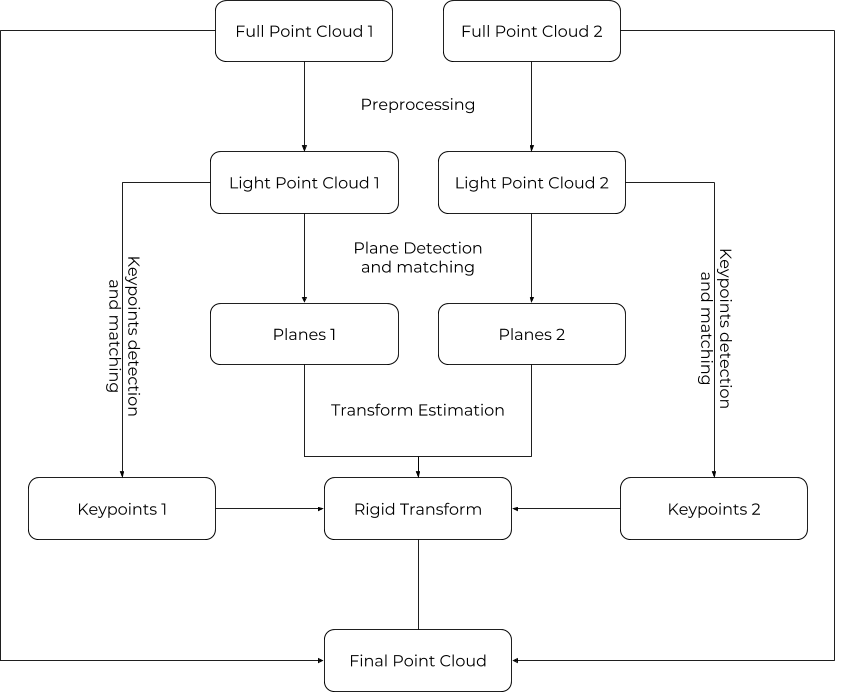
\includegraphics[scale=0.5]{images/pipeline.png}
    \caption{Registration pipeline.}
    \label{fig:pipeline}
\end{figure}
